\documentclass[man,floatsintext]{apa6}
\usepackage{lmodern}
\usepackage{amssymb,amsmath}
\usepackage{ifxetex,ifluatex}
\usepackage{fixltx2e} % provides \textsubscript
\ifnum 0\ifxetex 1\fi\ifluatex 1\fi=0 % if pdftex
  \usepackage[T1]{fontenc}
  \usepackage[utf8]{inputenc}
\else % if luatex or xelatex
  \ifxetex
    \usepackage{mathspec}
  \else
    \usepackage{fontspec}
  \fi
  \defaultfontfeatures{Ligatures=TeX,Scale=MatchLowercase}
\fi
% use upquote if available, for straight quotes in verbatim environments
\IfFileExists{upquote.sty}{\usepackage{upquote}}{}
% use microtype if available
\IfFileExists{microtype.sty}{%
\usepackage{microtype}
\UseMicrotypeSet[protrusion]{basicmath} % disable protrusion for tt fonts
}{}
\usepackage{hyperref}
\hypersetup{unicode=true,
            pdftitle={Cognitive correlates of mental health in adolescence: A network analysis approach},
            pdfauthor={Sam Parsons, Annabel Songco, Charlotte Booth, \& Elaine Fox},
            pdfkeywords={keywords},
            pdfborder={0 0 0},
            breaklinks=true}
\urlstyle{same}  % don't use monospace font for urls
\usepackage{graphicx,grffile}
\makeatletter
\def\maxwidth{\ifdim\Gin@nat@width>\linewidth\linewidth\else\Gin@nat@width\fi}
\def\maxheight{\ifdim\Gin@nat@height>\textheight\textheight\else\Gin@nat@height\fi}
\makeatother
% Scale images if necessary, so that they will not overflow the page
% margins by default, and it is still possible to overwrite the defaults
% using explicit options in \includegraphics[width, height, ...]{}
\setkeys{Gin}{width=\maxwidth,height=\maxheight,keepaspectratio}
\IfFileExists{parskip.sty}{%
\usepackage{parskip}
}{% else
\setlength{\parindent}{0pt}
\setlength{\parskip}{6pt plus 2pt minus 1pt}
}
\setlength{\emergencystretch}{3em}  % prevent overfull lines
\providecommand{\tightlist}{%
  \setlength{\itemsep}{0pt}\setlength{\parskip}{0pt}}
\setcounter{secnumdepth}{0}
% Redefines (sub)paragraphs to behave more like sections
\ifx\paragraph\undefined\else
\let\oldparagraph\paragraph
\renewcommand{\paragraph}[1]{\oldparagraph{#1}\mbox{}}
\fi
\ifx\subparagraph\undefined\else
\let\oldsubparagraph\subparagraph
\renewcommand{\subparagraph}[1]{\oldsubparagraph{#1}\mbox{}}
\fi

%%% Use protect on footnotes to avoid problems with footnotes in titles
\let\rmarkdownfootnote\footnote%
\def\footnote{\protect\rmarkdownfootnote}


  \title{Cognitive correlates of mental health in adolescence: A network analysis approach}
    \author{Sam Parsons\textsuperscript{1}, Annabel Songco\textsuperscript{1}, Charlotte Booth\textsuperscript{1}, \& Elaine Fox\textsuperscript{1}}
    \date{}
  
\shorttitle{Combined Cognitive Bias Hypothesis Network}
\affiliation{
\vspace{0.5cm}
\textsuperscript{1} University of Oxford}
\keywords{keywords\newline\indent Word count: X}
\usepackage{csquotes}
\usepackage{upgreek}
\captionsetup{font=singlespacing,justification=justified}

\usepackage{longtable}
\usepackage{lscape}
\usepackage{multirow}
\usepackage{tabularx}
\usepackage[flushleft]{threeparttable}
\usepackage{threeparttablex}

\newenvironment{lltable}{\begin{landscape}\begin{center}\begin{ThreePartTable}}{\end{ThreePartTable}\end{center}\end{landscape}}

\makeatletter
\newcommand\LastLTentrywidth{1em}
\newlength\longtablewidth
\setlength{\longtablewidth}{1in}
\newcommand{\getlongtablewidth}{\begingroup \ifcsname LT@\roman{LT@tables}\endcsname \global\longtablewidth=0pt \renewcommand{\LT@entry}[2]{\global\advance\longtablewidth by ##2\relax\gdef\LastLTentrywidth{##2}}\@nameuse{LT@\roman{LT@tables}} \fi \endgroup}


\usepackage{lineno}

\linenumbers
\usepackage{float}
\floatplacement{figure}{H}
\raggedbottom

\authornote{Add complete departmental affiliations for each author here. Each new line herein must be indented, like this line.

Enter author note here.

Correspondence concerning this article should be addressed to Sam Parsons, Postal address. E-mail: \href{mailto:sam.parsons@psy.ox.ac.uk}{\nolinkurl{sam.parsons@psy.ox.ac.uk}}}

\abstract{
This is my abstract


}

\begin{document}
\maketitle

\begin{table}[tbp]
\begin{center}
\begin{threeparttable}
\caption{\label{tab:table1}}
\begin{tabular}{lrrrrrrrrr}
\toprule
 & \multicolumn{1}{c}{mean} & \multicolumn{1}{c}{sd} & \multicolumn{1}{c}{       (1)} & \multicolumn{1}{c}{       (2)} & \multicolumn{1}{c}{       (3)} & \multicolumn{1}{c}{       (4)} & \multicolumn{1}{c}{       (5)} & \multicolumn{1}{c}{       (6)} & \multicolumn{1}{c}{       (7)}\\
\midrule
MH (1) & 40.72 & 12.58 &  &  &  &  &  &  & \\
IB\_S\_Pos (2) & 2.55 & 0.62 & .37 &  &  &  &  &  & \\
IB\_N\_Pos (3) & 3.53 & 0.64 & .33 & .40 &  &  &  &  & \\
IB\_S\_Neg (4) & 3.29 & 0.88 & -.25 & -.26 & -.17 &  &  &  & \\
IB\_N\_Neg (5) & 3.17 & 0.72 & -.15 & -.00 & -.19 & .51 &  &  & \\
MB\_Pos (6) & 6.83 & 2.87 & .40 & .30 & .21 & -.24 & -.15 &  & \\
MB\_Neg (7) & 2.50 & 2.34 & -.43 & -.28 & -.25 & .42 & .24 & -.29 & \\
\bottomrule
\end{tabular}
\end{threeparttable}
\end{center}
\end{table}

Background:

The data are drawn from the CogBIAS longitudinal study (wave 1 only). Analysed are the DVs from the interpretation bias task, memory bias task, and mental health questionnaire.

\hypertarget{comparing-groups-high-and-low-in-positive-mental-health}{%
\subsection{Comparing groups high and low in positive mental health}\label{comparing-groups-high-and-low-in-positive-mental-health}}

Figure 1 presents regularised partial correlations amongst interpretation and memory biases.

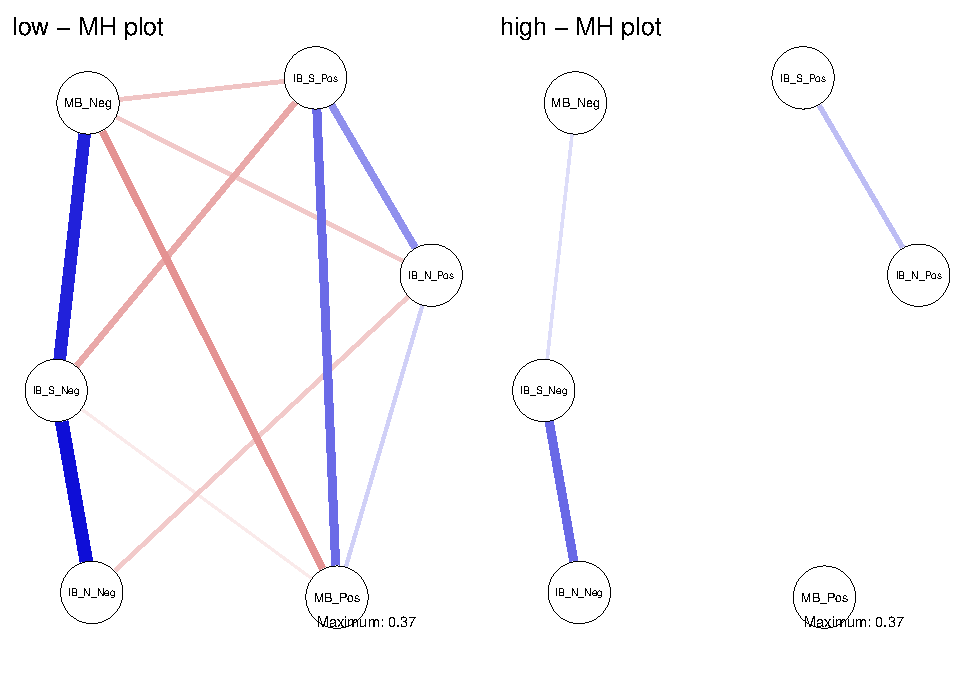
\includegraphics{script_files/figure-latex/plotting_highlow-1.pdf}

\hypertarget{network-comparisons}{%
\subsubsection{network comparisons}\label{network-comparisons}}

We compared the estimated networks using NetworkComparisonTest with 1000 iterations. Global strength in the high MH group (0.37) differed from that in the low MH group (1.70), \emph{p} = .015. There was no significant difference between global strength in the low MH group and the mid MH group (0.73).

\newpage

\hypertarget{including-mental-health-in-the-model}{%
\subsection{Including Mental Health in the model}\label{including-mental-health-in-the-model}}

We explored the difference in models between high and low groups using the mgm package. Figure 2 presents the network including mental health as a categorical variable (only for high and low MH groups).

Note. the shaded area of the \enquote{pie} is the predicability of that node, i.e.~the variance explained in that variable by the rest of the network. (I also need to include a more detailed explanation of why MH is different here as a categorical variable).

this network shows largely the same pattern as splitting by the high and low group. Some of the edges appear to be moderated by mental health.

\hypertarget{moderated-network}{%
\subsubsection{moderated network}\label{moderated-network}}

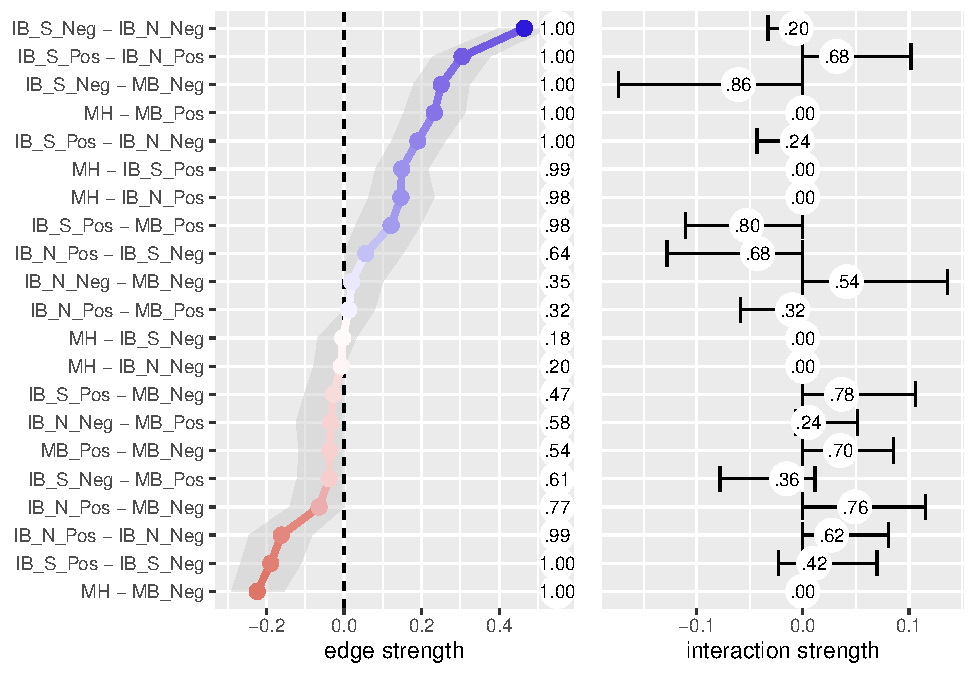
\includegraphics{script_files/figure-latex/plotting the moderated network interactions-1.pdf}

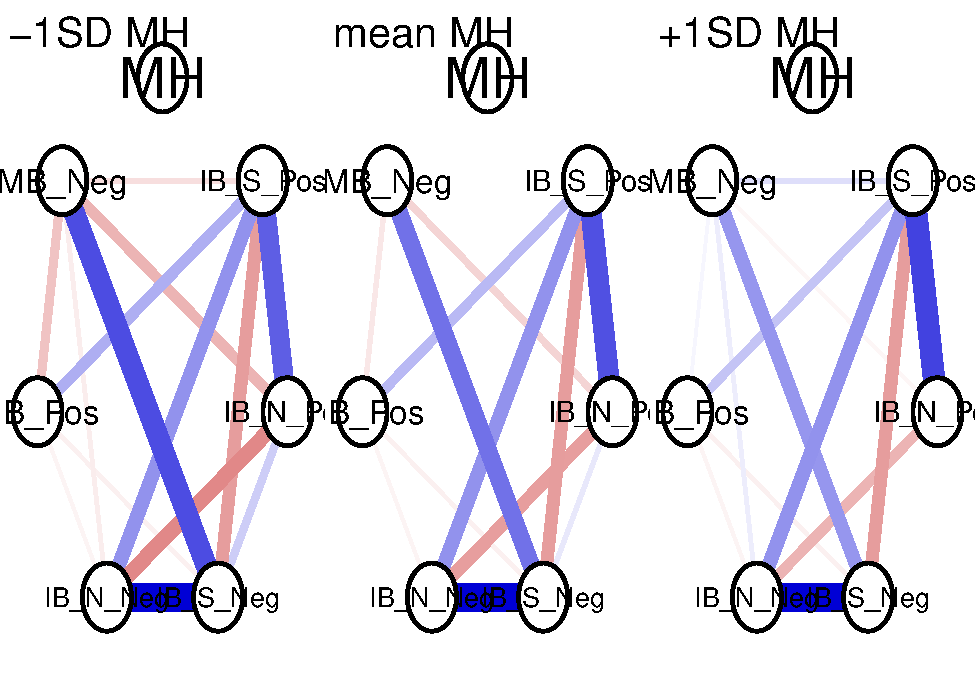
\includegraphics{script_files/figure-latex/conditioning the visualisations on mental health-1.pdf}

\newpage

\hypertarget{references}{%
\section{References}\label{references}}

\begingroup
\setlength{\parindent}{-0.5in}
\setlength{\leftskip}{0.5in}

\hypertarget{refs}{}

\endgroup


\end{document}
